\documentclass[a4paper]{report}
\usepackage[utf8]{inputenc}
\usepackage[T1]{fontenc}
\usepackage{RJournal}
\usepackage{amsmath,amssymb,array}
\usepackage{booktabs}


% tightlist command for lists without linebreak
\providecommand{\tightlist}{%
  \setlength{\itemsep}{0pt}\setlength{\parskip}{0pt}}


% Always define CSL refs as bib entries are contained in separate doc
% Pandoc citation processing
\newlength{\cslhangindent}
\setlength{\cslhangindent}{1.5em}
\newlength{\csllabelwidth}
\setlength{\csllabelwidth}{3em}
\newlength{\cslentryspacingunit} % times entry-spacing
\setlength{\cslentryspacingunit}{\parskip}
% for Pandoc 2.8 to 2.10.1
\newenvironment{cslreferences}%
  {}%
  {\par}
% For Pandoc 2.11+
\newenvironment{CSLReferences}[2] % #1 hanging-ident, #2 entry spacing
 {% don't indent paragraphs
  \setlength{\parindent}{0pt}
  % turn on hanging indent if param 1 is 1
  \ifodd #1
  \let\oldpar\par
  \def\par{\hangindent=\cslhangindent\oldpar}
  \fi
  % set entry spacing
  \setlength{\parskip}{#2\cslentryspacingunit}
 }%
 {}
\usepackage{calc}
\newcommand{\CSLBlock}[1]{#1\hfill\break}
\newcommand{\CSLLeftMargin}[1]{\parbox[t]{\csllabelwidth}{#1}}
\newcommand{\CSLRightInline}[1]{\parbox[t]{\linewidth - \csllabelwidth}{#1}\break}
\newcommand{\CSLIndent}[1]{\hspace{\cslhangindent}#1}



\begin{document}


%% do not edit, for illustration only
\sectionhead{Contributed research article}
\volume{XX}
\volnumber{YY}
\year{20ZZ}
\month{AAAA}

\begin{article}
  % !TeX root = RJwrapper.tex
\title{Tagtools: A tool for analyzing high resolution biologging data}


\author{by Yuqian wang and Oghenesuvwe Ogedegbe}

\maketitle

\abstract{%
An abstract of less than 150 words.
}

\hypertarget{introduction}{%
\section{Introduction}\label{introduction}}

Bio-logging studies, where data are collected using animal-borne devices, continue to grow rapidly in numbers and in scope. Data from high-resolution tags are essential for assessing marine mammal behavior in relation to acoustic disturbance, as well as for acquiring baseline behavior for environmental risk models. A subset of these tags include sensors for speed, turning rate (gyroscopes), and sound, increasing the array of inferences that can be drawn about the context and energetic cost of responses to disturbance. While these tags offer exciting opportunities to observe animal behavior in unprecedented detail, there is a desperate need for freely-available, easy-to-use, flexible software tools along with appropriate training to facilitate analysis and interpretation of the resulting data.

\hypertarget{background}{%
\section{Background}\label{background}}

High-resolution multi-sensor tags typically include accelerometers that are used to measure body orientation, sudden movement, changes in speed, and to estimate energy expenditure. These tags also use magnetometers to measure direction of travel, and pressure sensors to measure dive depth in aquatic or marine animals. A subset of tags also include sensors for speed, turning rate (gyroscopes), and sound (hydrophones), increasing researchers' ability to directly and indirectly assess impact from disturbances. These tags offer exciting opportunities to observe animal behavior in unprecedented detail and to quantify the consequences of human disturbance. However, analyses of the data are time-consuming and rely on a small cadre of highly-skilled scientists, creating a bottleneck in dissemination of these key findings.(Wilmers et al. 2015)

\hypertarget{processing}{%
\section{Processing}\label{processing}}

Through data processing we can extract meaningful inferences about animal behavior and patterns. We offer a range of functions to process the collected data for various purposes. These functions include automated sensor calibration, identification of dive start and end times, calculation of essential dive parameters (such as depth, duration, and kinematic parameters), analysis of movement patterns (such as residence index, straightness of movement, and tortuosity), evaluation of acceleration metrics (such as MSA, ODBA, and norm-jerk), and determination of acoustic characteristics (including standard measures of intensity, duration, bandwidth, and frequency for echolocation clicks or other relevant sounds). Notably, one prominent function is ``find\_dives,'' which locates time references for the initiation and conclusion of dives in a depth record or flights in an altitude record.By automating the process of finding these time cues, the function simplifies the analysis of large datasets, allowing researchers to focus on interpretations of these events.The simulated quantities used to do this are:

\begin{itemize}
\tightlist
\item
  p: A depth or altitude time series (a sensor data list or a vector) in meters.
\item
  sampling\_rate: The sampling rate of the sensor data in Hz (samples per second).
\item
  mindepth: The threshold in meters at which to recognize a dive or flight. Dives shallow or flights lower than mindepth will be ignored.
\item
  surface (optional): The threshold in meters at which the animal is presumed to have reached the surface. Default value is 1. A smaller value can be used if the dive/altitude data are very accurate and you need to detect shallow dives/flights.
\item
  findall (optional) When TRUE, forces the algorithm to include incomplete dives at the start and end of the record. Default is FALSE which only recognizes complete dives.
\end{itemize}

Find\_dives creates a data frame with one row for each dive or flight found. The columns of T are:
start (time in seconds of the start of each dive/flight)
end (time in seconds of the start of each dive/flight)
max (maximum depth/altitude reached in each dive/flight)
tmax(time in seconds at which the animal reaches the max depth/altitude).

Using the dataset beaked\_whale from the package as BW, the result produced are:

\begin{verbatim}
BW <- beaked_whale
find_dives(p = BW$P$data, sampling_rate = BW$P$sampling_rate, mindepth = 5, surface = 2, findall = FALSE)
\end{verbatim}

\begin{verbatim}
#>   start  end        max tmax
#> 1   178 3920 1086.99275 1400
#> 2  3987 4039    6.21215 4012
#> 3  4243 5293  238.84884 4692
\end{verbatim}

Alternating the number for the minimum depth produces different results with the number of dives shown, increasing, or decreasing. This information is crucial for understanding the behavior of the studied species. Researchers can experiment with different depth thresholds to discover optimal values that accurately capture relevant dives while minimizing false detections. This allows researchers to fine-tune their analysis and ensure that the results align with the specific research objectives and the characteristics of the organisms being studied.

For example, changing the value of mindepth to 1 would result in a dataframe of 19 rows:

\begin{verbatim}
find_dives(p = BW$P$data, sampling_rate = BW$P$sampling_rate, mindepth = 1, surface = 2, findall = FALSE)
\end{verbatim}

\begin{verbatim}
#>    start  end      max tmax
#> 1     52   54 1.105762   52
#> 2     61   63 1.128402   61
#> 3     82   84 1.106712   82
#> 4     99  101 1.122345  101
#> 5    109  111 1.116125  111
#> 6    122  124 1.127342  122
#> 7    138  140 1.142730  138
#> 8    149  151 1.097930  151
#> 9    176  178 1.197597  178
#> 10  3982 3984 1.090211 3984
#> 11  4148 4150 1.019758 4150
#> 12  4240 4242 1.055129 4242
#> 13  5308 5310 1.020068 5310
#> 14  5317 5319 1.098602 5319
#> 15  5327 5329 1.076354 5329
#> 16  5337 5339 1.075175 5339
#> 17  5346 5348 1.016802 5348
#> 18  5376 5378 1.093268 5378
#> 19  5381 5383 1.196322 5383
\end{verbatim}

Furthermore, to look at a more comprehensive view of the dive records available, we can look at the information presented using dive\_stats. The function dive\_stats() produces a profile of depth/altitude and a series of dive/flight start and end times. The simulated quantities for this are:

\begin{itemize}
\tightlist
\item
  P: Depth data in the form of a vector (or one-column matrix), or a tag sensor data list.
\item
  X (optional): Another data stream, as a vector (or a one-column matrix) or a tag sensor data list, for which to compute mean and variability. If angular is TRUE, it is interpreted as angular data (e.g., pitch, roll, or heading) with means and variances computed accordingly. The unit of measure must be in radians (not degrees). Currently, X must be regularly sampled.
\item
  dive\_cues: A two-column data frame or matrix with dive/flight start times in the first column and dive/flight end times in the second. Units should be in seconds since the start of tag recording. It may be obtained from find\_dives.
\item
  sampling\_rate (optional): The sampling rate of P (and X, if given). Ignored if P or X are tag sensor data lists. If omitted, the input data must be sensor data lists. If one value is given and both P and X are input, they are assumed to have the same sampling rate. If P and X have different sampling rates, this input can have two elements (first for P, second for X).
\item
  prop: The proportion of the maximal excursion to use for defining the ``destination'' phase of a dive or flight. For example, if prop is 0.85 (the default), then the destination phase lasts from the first to the last time depth/altitude exceeds 0.85 times the within-dive maximum.
\item
  angular: Is X angular data? Defaults to FALSE.
\item
  X\_name: A short name to use for the X variable in the output data frame. For example, if X is pitch data, use X\_name=`pitch' to get output column names like mean\_pitch, etc. Defaults to `angle' for angular data and `aux' for non-angular data.
\item
  na.rm: Logical, default is TRUE. If TRUE, then returned mean values ignore missing values, computing an average over all non-missing observations.
\end{itemize}

Dive\_stats() returns a data frame that contains information about each dive or flight excursion. Each row in the data frame corresponds to one dive or flight, and the columns provide various details about the excursion. All time-related values are in seconds, and rates are expressed in units of x/sec, where x represents the units of the input \texttt{P} parameter.

The columns included in the data frame are as follows:

\begin{itemize}
\tightlist
\item
  max: Represents the maximum depth or altitude reached during the excursion.
\item
  st: Denotes the start time of the dive or flight in seconds, obtained from the input \texttt{dive\_cues}.
\item
  et: Indicates the end time of the dive or flight in seconds, also obtained from the input dive\_cues.
\item
  dur: Represents the total duration of the excursion in seconds.
\item
  dest\_st: Represents the start time of the destination phase in seconds since the start of tag recording. This time also marks the end time of the ``to'' phase within the dive or flight.
\item
  dest\_et: Represents the end time of the destination phase in seconds since the start of tag recording. This time also marks the start time of the ``from'' phase within the dive or flight.
\item
  dest\_dur: Denotes the duration of the destination phase in seconds.
\item
  to\_dur: Denotes the duration of the ``to'' phase within the dive or flight in seconds.
\item
  from\_dur: Denotes the duration of the ``from'' phase within the dive or flight in seconds.
\end{itemize}

Depending on the parameters used, additional columns may be present in the data frame:

\begin{itemize}
\tightlist
\item
  mean\_angle: If angular=TRUE and X is provided as input, this column represents the mean angle for the entire excursion. Separate columns (mean\_to\_angle, mean\_dest\_angle, and mean\_from\_angle) provide mean angles for each phase within the dive or flight.
\item
  angle\_var: If angular=TRUE and X is provided as input, this column represents the angular variance for the entire excursion. Separate columns (to\_angle\_var, dest\_angle\_var, and from\_angle\_var) provide angular variances for each phase within the dive or flight.
\item
  mean\_aux: If angular=FALSE and X is provided as input, this column represents the mean value of X for the entire excursion. Separate columns (mean\_to\_aux, mean\_dest\_aux, and mean\_from\_aux) provide mean values of X for each phase within the dive or flight.
\item
  aux\_sd: If angular=FALSE and X is provided as input, this column represents the standard deviation of X for the entire excursion. Separate columns (to\_aux\_sd, dest\_aux\_sd, and from\_aux\_sd) provide standard deviations of X for each phase within the dive or flight.
\end{itemize}

Dive\_stats is to be used in conjunction with find\_dives to provide more information on dives that have already been identified. Using the ZC dataset obtained from ``zc11\_267a.nc'' nc file, we can plot a dive profile and choose a suitable chunk to analyze.

\begin{verbatim}
path <- "../vignettes/articles/nc_files/zc11_267a.nc"
ZC <- load_nc(path)

plott(X=list(Depth=ZC$P), r = TRUE)
\end{verbatim}

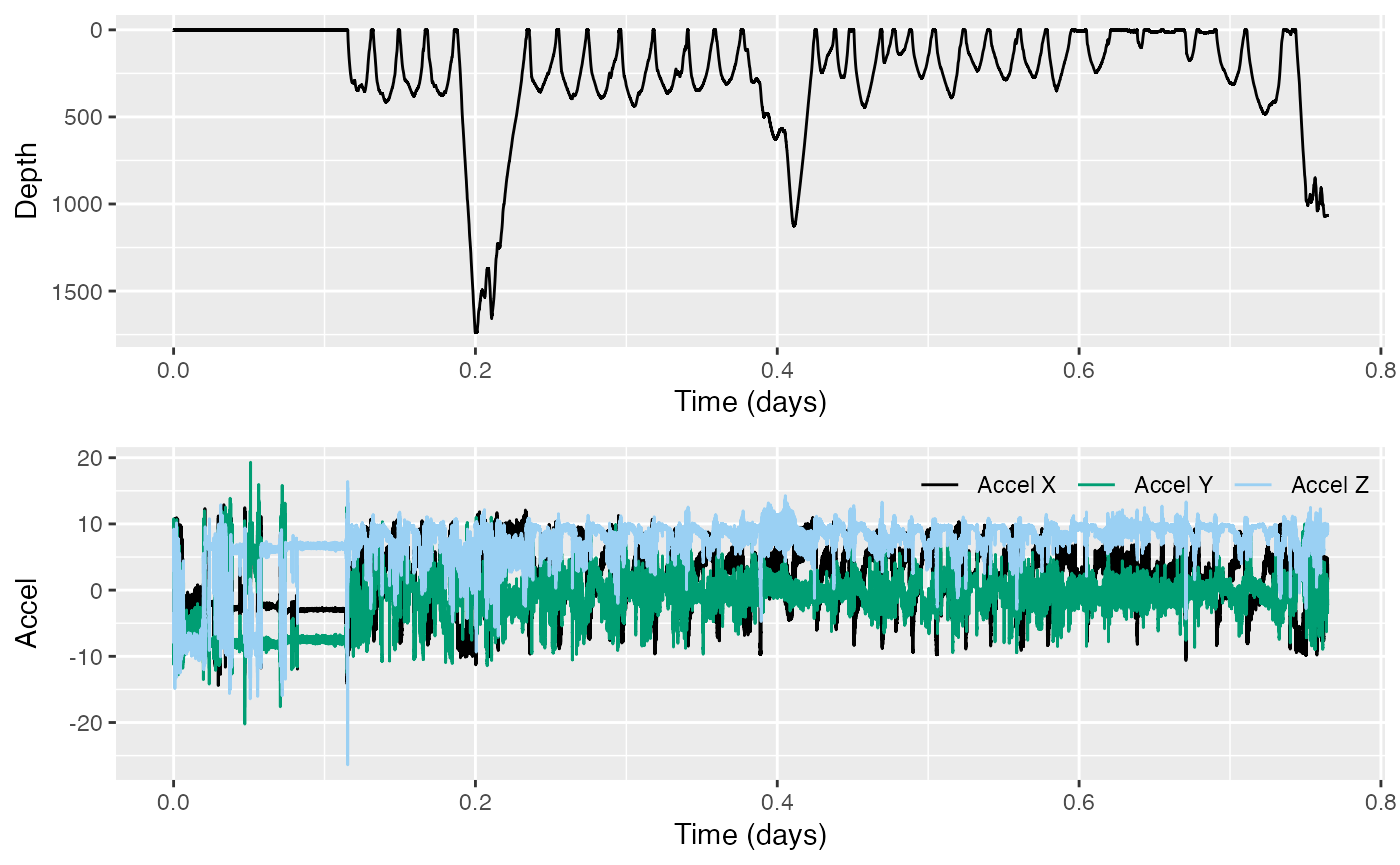
\includegraphics{journal_files/figure-latex/unnamed-chunk-3-1.pdf}

With the plot in view we can choose a suitable depth to find dives for.

\begin{verbatim}
d <- find_dives(ZC$P,500) 
\end{verbatim}

We can further crop the plot to find information on particular waves. Here we can look at the first two waves and see what dive\_stats produces as a result.

\begin{verbatim}
P <- crop_to(ZC$P, tcues = c(d$start[1], d$end[2]))

dive_stats(P, dive_cues=d[,c('start', 'end'),])
\end{verbatim}

\begin{verbatim}
#>   num      max      st      et    dur dest_st dest_et dest_dur to_dur from_dur
#> 1   1 1125.833 16151.8 20229.6 4077.8 19163.2 19639.4    476.2 3011.4    590.4
#> 2   2     -Inf 32580.0 36711.4 4131.4     Inf    -Inf     -Inf    Inf      Inf
#>     to_rate  from_rate
#> 1 0.2769636 -0.9771842
#> 2        NA         NA
\end{verbatim}

Two other functions that are of particular interest in terms of data processing are msa() and odba().

The Msa() function is used to compute the Minimum Specific Acceleration (MSA). This is the absolute value of the norm of the acceleration minus 1 g, i.e., the amount that the acceleration differs from the gravity value. This is always equal to or less than the actual specific acceleration if A is correctly calibrated. Should MSA exceed the expected range, there is a clear potential for inaccurate measurements. The simulated quanties for this function are:

\begin{itemize}
\item
  A: An nx3 acceleration matrix with columns {[}ax ay az{]}, or a tag sensor data list containing acceleration data. Acceleration can be in any consistent unit, e.g., g or m/s\^{}2. A can be in any frame as the MSA is rotation independent.
\item
  ref: The gravitational field strength in the same units as A. This parameter is not needed if A is a sensor structure. If A is a matrix, the default value is 9.81, assuming that A is in m/s\^{}2. Use ref = 1 if the unit of A is g.
\end{itemize}

The result of running it on a suitable dataset is a column vector of MSA with the same number of rows as A, or a tag sensor data list (output matches input). The MSA values (m) have the same units as A (e.g., g or m/s\^{}2).

\begin{verbatim}
msa(ZC$A)$data[1:18]
\end{verbatim}

\begin{verbatim}
#>  [1] 1.0386814 1.9996153 1.1563563 1.1778072 0.1246457 0.6830216 1.8871394
#>  [8] 0.9207138 0.1500726 0.8410105 0.9207391 0.7463868 1.7783814 1.1383616
#> [15] 1.6107005 0.1414111 1.3126264 0.9320780
\end{verbatim}

Similarly to msa(), odba is another function used to analyze acceleration data. ODBA stands for ``Overall Dynamic Body Acceleration'' as defined by Wilson et al.~in 2006. This is derived from the norm of the high-pass-filtered acceleration taken from animal tags. arious methods for computing ODBA exist, differing in the choice of norm and filter used.

In the Wilson paper, the 1-norm and a rectangular window (moving average) filter are employed. The high-pass filter is implemented by subtracting the moving average from the input accelerations.

Alternatively, the 2-norm, also known as VeDBA, may be preferred if the tag orientation is unknown or subject to change. For VeDBA, a tapered symmetric FIR filter is used for more efficient high-pass filtering compared to the rectangular window method, effectively avoiding lobes in the response.

The simulated quantities for calculating odba are:

\begin{itemize}
\tightlist
\item
  A: A tag sensor data list containing tri-axial acceleration data or an nx3 acceleration matrix with columns {[}ax ay az{]}. Acceleration can be in any consistent unit, e.g., g or m/s\^{}2. A can be in any frame, but the result depends on the method used to compute ODBA.
\item
  sampling\_rate: The sampling rate in Hz of the acceleration signals. Required for the `fir' method if A is not a tag sensor data list.
\item
  fh: The high-pass filter cut-off frequency in Hz. This should be chosen to be about half of the stroking rate for the animal (e.g., using dsf.R). Required for the default `fir' method.
\item
  method: A character containing either `wilson' or `vedba' or `fir'. This determines the method by which the ODBA is calculated. The default method is `fir'.
\item
  n: The rectangular window (moving average) length in samples. This is only needed if using the classic ODBA and VeDBA forms (methods `wilson' and `vedba').
\end{itemize}

A column vector of ODBA is returned with the same number of rows as A. ODBA values have the same units as A

\begin{verbatim}
odba(A = ZC$A$data, sampling_rate = ZC$A$sampling_rate, fh = 0.05)[1:18]
\end{verbatim}

\begin{verbatim}
#>  [1] 2.644054 3.779015 3.079952 3.255186 2.285308 2.850576 4.192403 3.367263
#>  [9] 2.288785 3.532974 4.054720 4.240424 5.623113 5.225649 5.759661 4.893031
#> [17] 2.589384 5.070509
\end{verbatim}

\hypertarget{calibration}{%
\section{Calibration}\label{calibration}}

\begin{verbatim}
Biologging tags, such as accelerometers, and gyroscopes, provide strong insight into the behavior of animals, but their measurements can be influenced by various external factors such as environmental conditions and sensor bias. As such, calibration is required to correct any errors or inconsistencies in the collected data. By comparing the measurements obtained from the biologging tags with known data, researchers can adjust the readings to improve accuracy of recorded data. This improves the process of analysis and interpretion of the data, which will result in more accurate conclusions to be drawn about the species being studied. Calibration is a key part in enesuring data integrity.
\end{verbatim}

\hypertarget{plotting}{%
\section{Plotting}\label{plotting}}

\begin{verbatim}
The main use of our package is to provide a comprehensive set of options for visualizing various behavioral metrics, such as activity levels, movement patterns, dive depths and duration. This streamlines the analysis process and helps researchers to better understand animal behavior. An important first step in tag data analysis is to plot the data.  Surprisingly, some of the most useful types of figures can be particularly hard to produce.  Examples include time-series plots that show several tag-sensor data streams in plot panels stacked atop one another, with all panels sharing a common time scale; or plots where sensor data from many exemplars of an event of interest are overlaid, in order to compare behavior between events. The resulting figures often prove crucially convincing to summarize results and complement statistical analysis in scientific publications. Unfortunately, since they are difficult to produce, creating them slows the pace of analysis (or they may even be neglected entirely).
\end{verbatim}

\hypertarget{sound-processing}{%
\section{Sound processing}\label{sound-processing}}

\begin{verbatim}
The package also undertakes some sound processing by way of measuring spectrum levels, plotting spectrograms and obtaining audio in the form of wav files. Sound speed is measured to ascertain the depth and position of the animal. 
\end{verbatim}

\hypertarget{summary}{%
\section{Summary}\label{summary}}

We have displayed various tooltips that are available in the package \pkg{ToOoOlTiPs}.

\hypertarget{references}{%
\section*{References}\label{references}}
\addcontentsline{toc}{section}{References}

\hypertarget{refs}{}
\begin{CSLReferences}{1}{0}
\leavevmode\vadjust pre{\hypertarget{ref-wilmers_golden_2015}{}}%
Wilmers, Christopher C., Barry Nickel, Caleb M. Bryce, Justine A. Smith, Rachel E. Wheat, and Veronica Yovovich. 2015. {``The Golden Age of Bio-Logging: How Animal-Borne Sensors Are Advancing the Frontiers of Ecology.''} \emph{Ecology} 96 (7): 1741--53. \url{https://doi.org/10.1890/14-1401.1}.

\end{CSLReferences}

\bibliography{references.bib}

\address{%
Yuqian wang\\
Calvin University\\%
Department of Letter Q\\ Somewhere, Australia\\
%
\url{https://www.britannica.com/animal/quokka}\\%
\textit{ORCiD: \href{https://orcid.org/0000-1721-1511-1101}{0000-1721-1511-1101}}\\%
\href{mailto:qquo@ulm.edu}{\nolinkurl{qquo@ulm.edu}}%
}

\address{%
Oghenesuvwe Ogedegbe\\
Calvin University\\%
Department of Letter Q, Somewhere, Australia\\ Department of Marsupials, Somewhere, Australia\\
%
\url{https://www.britannica.com/animal/bilby}\\%
\textit{ORCiD: \href{https://orcid.org/0000-0002-0912-0225}{0000-0002-0912-0225}}\\%
\href{mailto:bbil@ulm.edu}{\nolinkurl{bbil@ulm.edu}}%
}

\end{article}


\end{document}
